\chapter{Display Pages}
\label{Chapter10}
The software product contains two GUI pages. Main display page (status and selection page) and second display page (plotting page).
Main display page as shown in \ref{FIG:DPSMainPage} provides status of different sub-systems, functionality of different add on cards along with threads running status, various log counters, packets counters for MCC and RSP, pushbuttons for selections (logging, timing information, CDM sources) and enabling of plotting in secondary GUI along with switch over option to 2nd GUI page. \newline

Second display play is divided into four segments and is provided with a pushbutton for switching over to main GUI page. This second GUI page is shown in \ref{FIG:DPSSecondPage}. Segments are arranged in an array of 2$\times$2. At (0,0) azimuth response is plotted containing commanded angle and antenna position on primary y-axis and corresponding error on secondary y-axis. The plotting is done with reference to CDT on x-axis. Similarly, at (0,1) elevation response is plotted containing commanded angle and antenna position on primary y-axis and corresponding error on secondary y-axis. The plotting is done with reference to CDT on x-axis. Transmitter RF output power level status is displayed on primary y-axis with reference to CDT on x-axis and this is plotted in segment (1,0). Finally, the segment (1,1) contains radiated command word status on y-axis with reference to CDT on x-axis.

\begin{figure}[H]
	\centering
	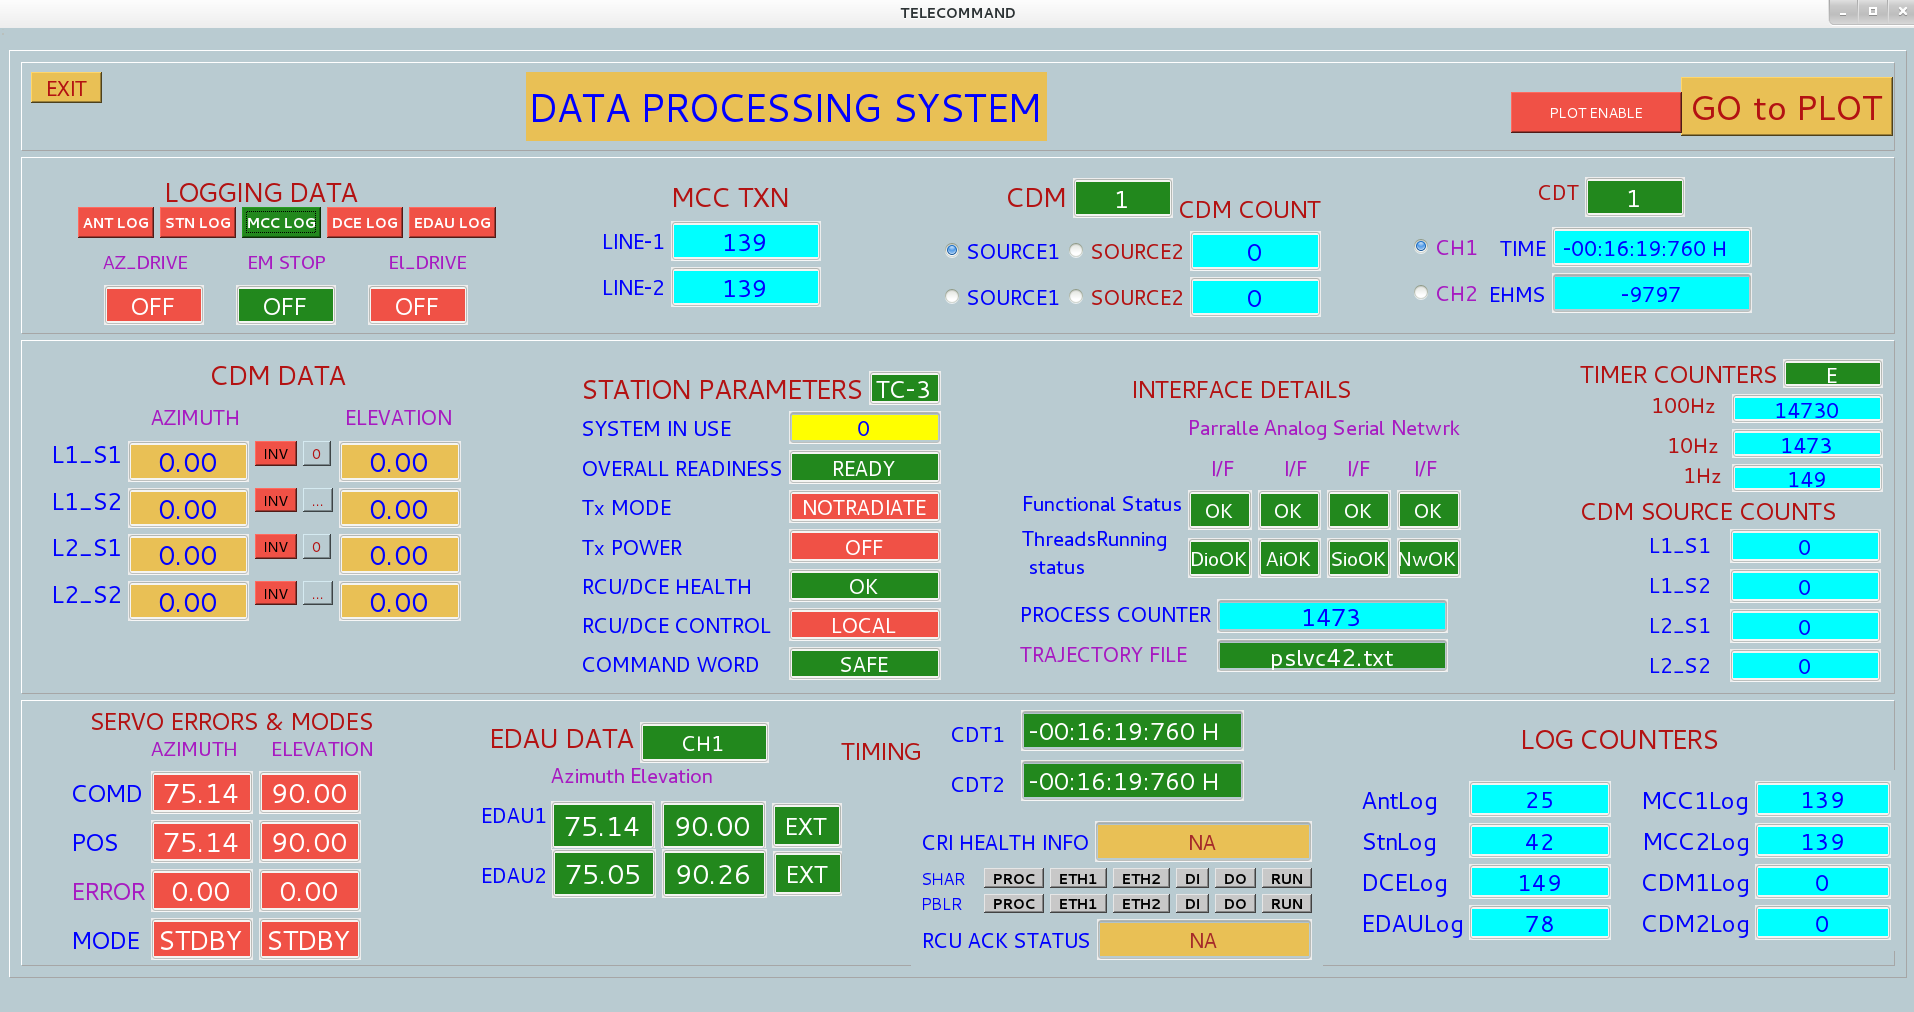
\includegraphics[height=1.2\linewidth, width=\linewidth]{./Diagrams/MainPage.png}
	\caption{DPS Main Page}
	\label{FIG:DPSMainPage}
\end{figure}
	   

\begin{figure}[H]
	\centering
	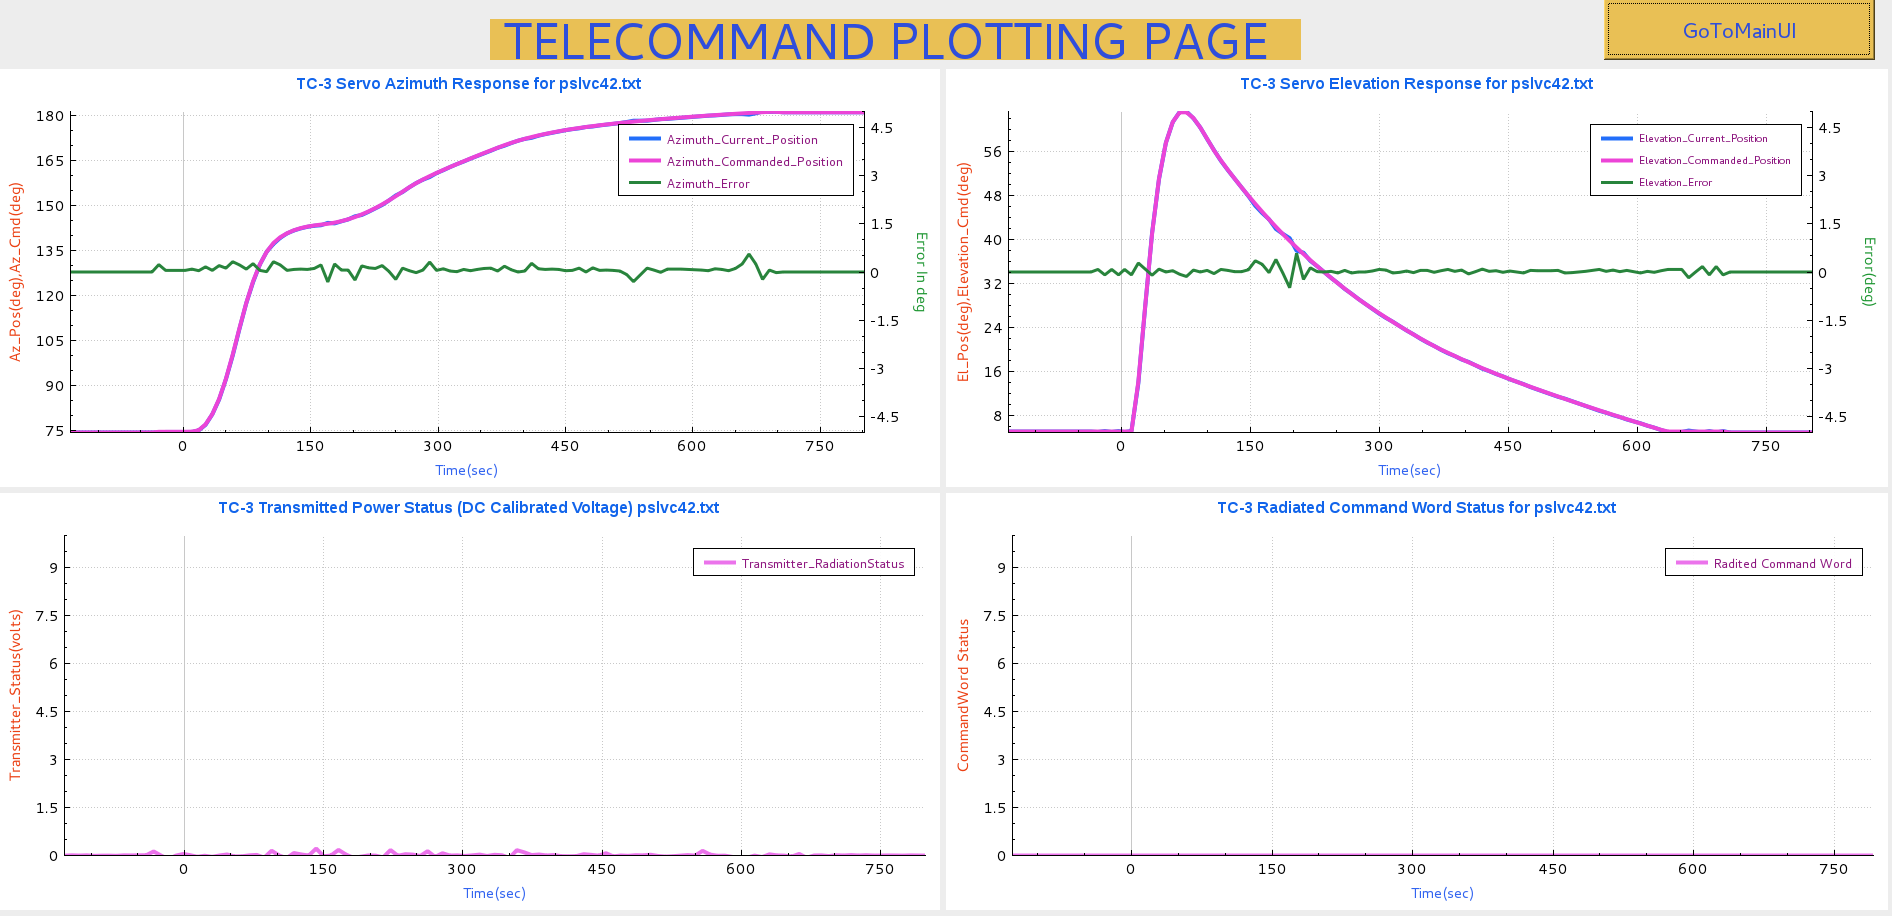
\includegraphics[height=1.2\linewidth, width=\linewidth]{./Diagrams/SecondaryPage.png}
	\caption{DPS Secondary Page}
	\label{FIG:DPSSecondPage}
\end{figure}